\section{Characteristic parameters}
The main method of stability testing is to check the values of multiple parameters in different runs and determine the abnormal runs by comparison. The most important characteristic parameters of testing is the invariant mass distribution of all out-going particles. The other parameters, such as photon number recorded by different ECALs, can also be used for the diagnosis of abnormalities. In the following subsections, different parameters are investigated for each run:

\begin{figure*}[!ht]
	\centering
	\begin{subfigure}[b]{0.49\textwidth}
		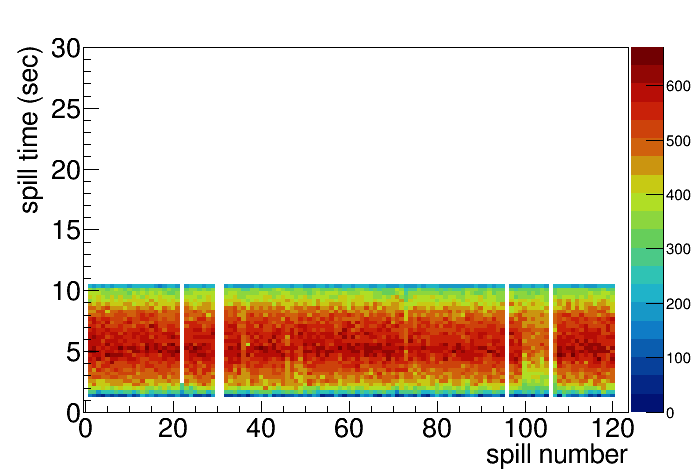
\includegraphics[width=\textwidth]{event_spill_70171}
		\caption{Run number 70171}
		\label{fig:EveN_spill_normal}
	\end{subfigure}
	~ %add desired spacing between images, e. g. ~, \quad, \qquad, \hfill etc. 
	%(or a blank line to force the subfigure onto a new line)
	\begin{subfigure}[b]{0.49\textwidth}
		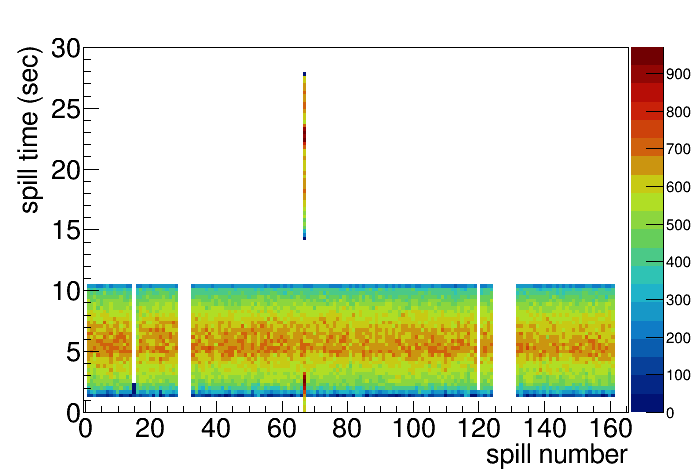
\includegraphics[width=\textwidth]{strange_spill_70195}
		\caption{Run number 70195}
		\label{fig:EveN_spill_abnormal}
	\end{subfigure}
	\caption{Temporal distribution of event numbers for each spill number. The color band represents the number of events per 0.3 seconds (time resolution) for each spill. The y axes represent the time from starting moment of each spill. (a) A normal temporal distribution (run number = 70171). The effective time expansion of particle beam is around 9s and distribution of each spill is centrally concentrated. (b) An abnormal temporal distribution (run number = 70195). Particle beam occurred in inactive time period.}
	\label{fig:animals}
\end{figure*}

\begin{figure*}[!h]
	\centering
	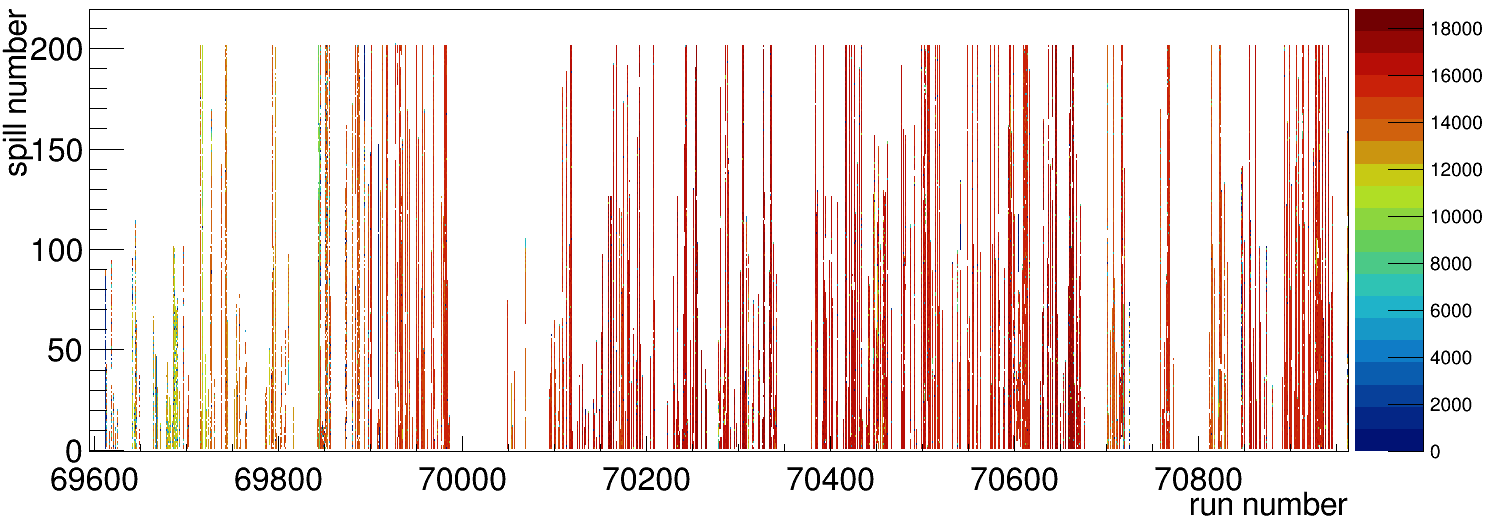
\includegraphics[width=\textwidth]{event_distribution_all}
	\caption{Event distribution with respect to spill number of each run number. The color band shows the value of event counting in certain spill of certain run. The run number ranging from $69595 \sim 70963$ while the maximal of spill number cannot exceed above 200. The number of events can goes up to 18000 per spill whereas it could also amount to only few thousands or less, especially in the beginning of experiment. }
	\label{fig:event_distribution_all}
\end{figure*}

\subsection{Number of events}
The number of events for each run can be vastly different after the preselection. By using PHAST data analysis framework, the event number for each spill of every run is counted and plotted. Since incoming particle beam only exist in certain time interval of spill, event numbers are not spread throughout whole time period of the spill. From the figure \ref{fig:EveN_spill_normal}, one can easily see that normally events are only distributed on the time interval \SI{1.2}{\second} $\sim$ \SI{10.5}{\second} of the spill period. There is a short dead period of \SI{1.2}{\second} before the start of particle beam and a long inactive period after the stop of beam at \SI{10.5}{\second} until the end of spill (at around \SI{48}{\second}). However, as is shown in figure \ref{fig:EveN_spill_abnormal}, there exists one abnormal run, where the effective time interval of one spill is more than 2 times larger than the normal one. This shows that the particle beam occurs during the inactive time interval not only right at the beginning of spill (\SI{0}{\second} $\sim$ \SI{1.2}{\second}), but also after the first stop of beam (\SI{14.1}{\second} $\sim$ \SI{27.9}{\second}). Such abnormality could probably result from the trigger problem, due to which events are recorded with wrong time scale.

After selecting out the run with abnormal temporal distribution discussed above, the number of events can be compared for each spill in every run, as is shown in figure \ref{fig:event_distribution_all}. The event number distribution is quite uneven throughout the experiment after the preselection. Runs in the beginning usually have low values of event counting and most of them don't have any event in some spills. Moreover, there exist large number of vacant runs with no events in all spills. Therefore, one can consider the number of events of each run as one of the characteristic parameters to test the stability of experiment. However, analyses such as invariant mass of three pion mass are independent from the number of events one have for each run. Thus, the variation of event distribution throughout the experiment could have little or no effect towards results of the analyses.

\subsection{Vertex positions}
The next parameter that could be investigated is the position of vertices. The location of vertices cannot be measured directly from the detectors but rather reconstructed by the charged particle tracks. When extracting the vertex position of the event by PHAST, there are only two types of vertices: primary vertices and non-primary vertices. The method of determining the vertices is by comparing tracks and find the intercept point between two reconstructed tracks. If this intercept point also lies on the track of incoming particle, it will be considered as a primary vertex. If not, it will be considered as non-primary vertex. 

\begin{figure}[!b]
	\centering
	\begin{subfigure}[t]{0.5\textwidth}
		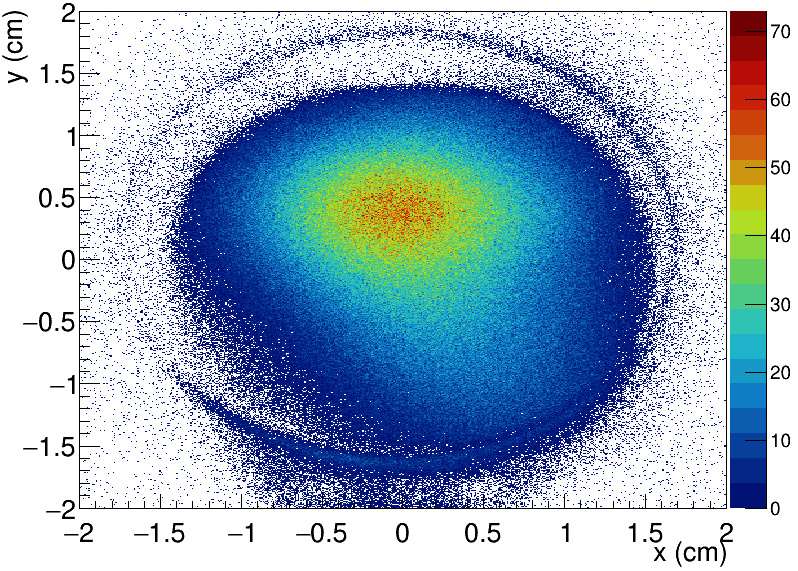
\includegraphics[width=\textwidth]{Prim_vertex_70171}
		\caption{Primary vertex positions}
		\label{fig:Prim_vertex_70171}
	\end{subfigure}
	~ %add desired spacing between images, e. g. ~, \quad, \qquad, \hfill etc. 
	%(or a blank line to force the subfigure onto a new line)
	\begin{subfigure}[b]{0.5\textwidth}
		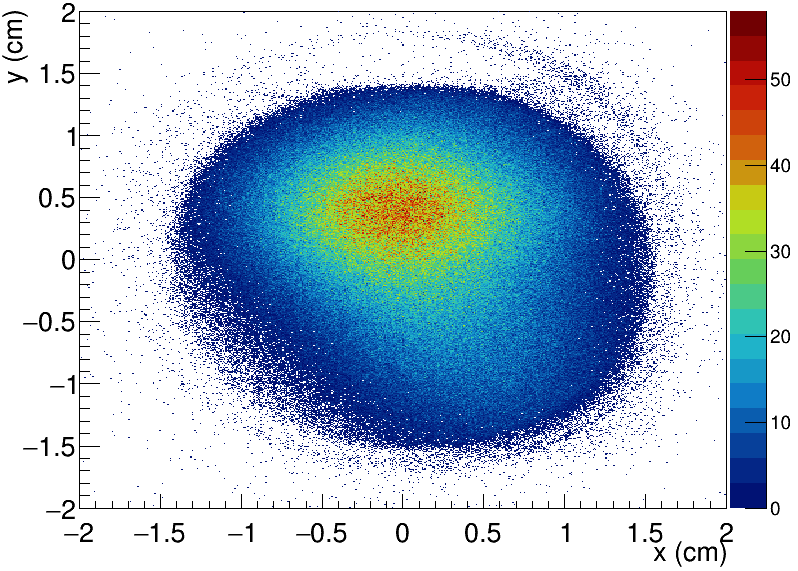
\includegraphics[width=\textwidth]{sec_vertex_70171}
		\caption{Non-primary vertex positions}
		\label{fig:sec_vertex_70171}
	\end{subfigure}
	\caption{vertex position distribution in x-y plane (z is the direction of the particle beam). The color band represents the number of vertices in corresponding location. Spacial resolution of x and y are both \SI{0.008}{\centi\meter}. (a) Distribution of primary vertices, in which a strange halo structure appears in the graph. (b) Distribution of non-primary vertices, where the halo disappears.}
	\label{fig:ver_pos}
\end{figure}

As has been discussed in subsection \ref{subsec:data_preselection}, the events after preselection contain either one charged track or three charged tracks. Event containing one charged track corresponds to elastic scattering while event with three charged tracks to inelastic scattering. In case of elastic scattering, since there is only one out-going particle track and one incoming particle track, all vertices being reconstructed are primary vertices. On the other hand, non-primary vertices could exists in inelastic scattering. This can be better explained by vertices position in figure \ref{fig:ver_pos}. The first graph, figure \ref{fig:Prim_vertex_70171}, shows the primary vertex position. As one can easily see, most of the vertex positions are on the liquid hydrogen target, which located at around $\SI{-1.4}{\centi\meter} \sim \SI{1.5}{\centi\meter}$ in x direction and $\SI{-1.5}{\centi\meter} \sim \SI{1.3}{\centi\meter}$ in y direction. Additional, there is halo shaped vertex points surrounding the target. The reason behind this strange shape is the elastic scattering between the $\pi$ beam and container of liquid hydrogen. From the vertices distribution on the target region, one can see that the particle density of the beam is Gaussian distributed in the cross section. There are more incoming particles in the central area of the beam than the peripheral area, leading to the decreasing the vertex number in the outward direction. But when the beam hits the metallic container, the vertex number surges due to the increase of elastic scattering cross-section between $\pi$ and metallic nucleus. Therefore, the vertices on the halo are most likely to be the primary vertices. This can be further proved when one checks the position of non-primary vertices. In figure \ref{fig:sec_vertex_70171}, the strange halo structure disappears, which indicates that most of events with three out-going particles corresponds to the inelastic scattering between the pion beam and hydrogen target.  

\subsection{Three pions invaraint mass}
The most obvious parameter that can be used to determine the instability should be the invariant mass distribution of three out-going pions of each run. 

\begin{figure*}[!t]
	\centering
	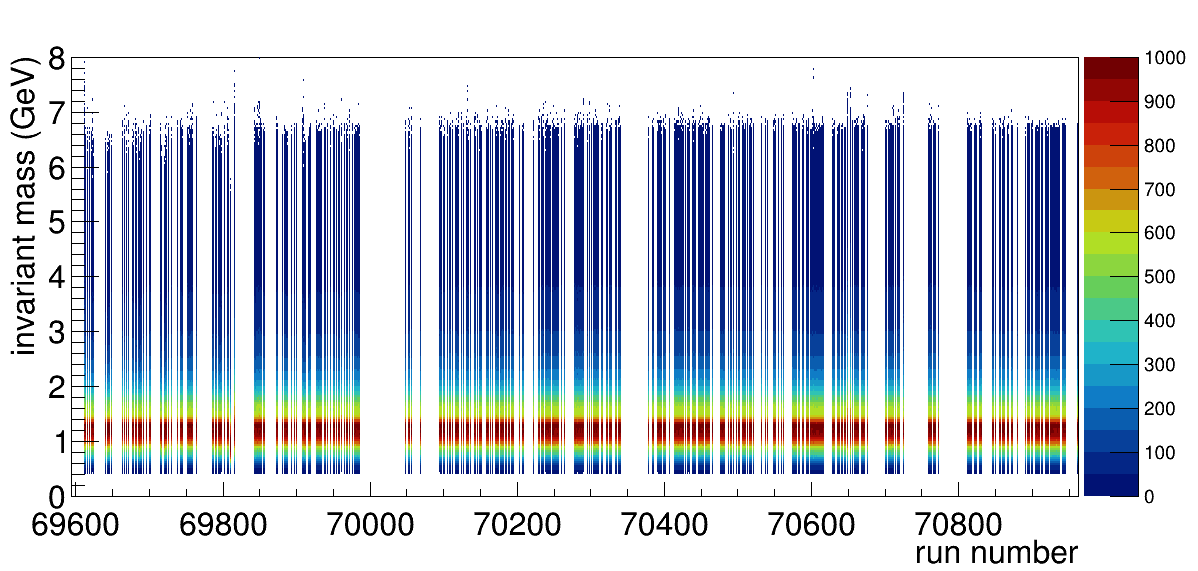
\includegraphics[width=\textwidth]{Three_pion_mass_his}
	\caption{Event distribution with respect to spill number of each run number. The color band shows the value of event counting in certain spill of certain run. The run number ranging from $69595 \sim 70963$ while the maximal of spill number cannot exceed above 200. The number of events can goes up to 18000 per spill whereas it could also amount to only few thousands or less, especially in the beginning of experiment. }
	\label{fig:Three_pion_mass_his}
\end{figure*}


\begin{figure*}[!t]
	\centering
	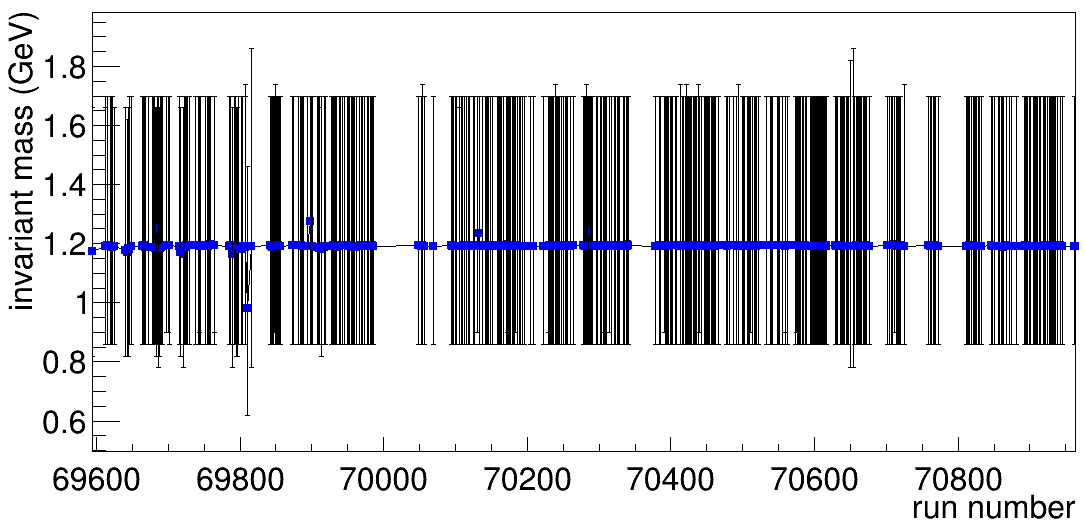
\includegraphics[width=\textwidth]{Three_pion_mass_Graph}
	\caption{Event distribution with respect to spill number of each run number. The color band shows the value of event counting in certain spill of certain run. The run number ranging from $69595 \sim 70963$ while the maximal of spill number cannot exceed above 200. The number of events can goes up to 18000 per spill whereas it could also amount to only few thousands or less, especially in the beginning of experiment. }
	\label{fig:Three_pion_mass_Graph}
\end{figure*}
\subsection{Photon and energy cut}
\subsection{Total invariant mass}
\subsection{Recoil proton}


\clearpage